%----------------------------------------------------------------------------------------
%    PACKAGES AND THEMES
%----------------------------------------------------------------------------------------
\documentclass[aspectratio=169,xcolor=dvipsnames]{beamer}
\makeatletter
\def\input@path{{theme/}}
\makeatother
\usetheme{CleanEasy}
\usepackage[utf8]{inputenc}
\usepackage{lmodern}
\usepackage[T1]{fontenc}
\usepackage{kotex}
\usepackage{fix-cm}
\usepackage{amsmath}
\usepackage{mathtools}
\usepackage{listings}
\usepackage{xcolor}
\usepackage{hyperref}
\usepackage{graphicx}
\usepackage{booktabs}
\usepackage{tikz}
\usetikzlibrary{positioning, shapes, arrows, calc, decorations.pathreplacing, arrows.meta, backgrounds, patterns, overlay-beamer-styles}
\usepackage{etoolbox}

%----------------------------------------------------------------------------------------
%    LAYOUT CONFIGURATION
%----------------------------------------------------------------------------------------



% Configure code listings
\lstset{
  basicstyle=\ttfamily\small,
  keywordstyle=\color{blue},
  commentstyle=\color{green!60!black},
  stringstyle=\color{red},
  showstringspaces=false,
  breaklines=true,
  frame=single,
  rulecolor=\color{black!30},
  backgroundcolor=\color{black!5},
  numbers=left,
  numberstyle=\tiny\color{black!70},
  numbersep=5pt
}


%----------------------------------------------------------------------------------------
%    TITLE PAGE CONFIGURATION
%----------------------------------------------------------------------------------------
\title[AI 활용 수업자료 생성]{AI를 활용한 수업자료 자동 생성 시스템}
\subtitle{강의 슬라이드 및 과제 생성 자동화}
\author{전민석}
\institute{DGIST}
\date{\today}

%----------------------------------------------------------------------------------------

\begin{document}

\begin{frame}[plain]
  \titlepage
\end{frame}

% \begin{frame}[plain]{목차}
%   \tableofcontents
% \end{frame}

%----------------------------------------------------------------------------------------
% \section{Why}
%----------------------------------------------------------------------------------------

\begin{frame}{배경 및 필요성}
  \begin{block}{현재의 문제점}
    \begin{itemize}
      \item 강의를 위한 \textbf{책, 강의자료(슬라이드), 과제의 수동 제작}에는 많은 시간과 노력이 요구됨
      \item 최신 지식 반영과 학생 맞춤형 자료 제공에 한계가 있음
    \end{itemize}
  \end{block}

  \vspace{0.5cm}

  \begin{exampleblock}{AI 활용의 이점}
    \begin{itemize}
      \item 강의 주제에 적합한 \textbf{강의자료의 초안을 신속하게 생성}
      \item 교수자가 검토 및 수정함으로써 고품질 교육 자료를 효율적으로 완성
      \item \textbf{슬라이드 제작 자동화, 과제 자동 생성} 등 다양한 교육 상황에 빠르고 유연하게 대응
    \end{itemize}
  \end{exampleblock}
\end{frame}

%----------------------------------------------------------------------------------------
% \section{목표 및 수행방법}
%----------------------------------------------------------------------------------------

% \begin{frame}{목표}
%   \begin{center}
%     \Large
%     \textbf{AI를 활용해 수업에서 사용할\\강의 슬라이드 및 과제를 생성하는 것이 목표}
%   \end{center}

%   \vspace{1cm}

%   \begin{block}{3단계 프로세스}
%     AI 기반 수업자료 생성을 위한 체계적인 접근
%   \end{block}
% \end{frame}

\begin{frame}{수행방법: 3단계 프로세스}
  \begin{center}
    \begin{tikzpicture}[
      box/.style={rectangle, rounded corners, draw=blue!50, fill=blue!10, thick, minimum height=2.5cm, minimum width=3.5cm, align=center},
      arrow/.style={->,>=stealth,thick}
    ]
      % Boxes
      \node[box] (step1) at (0,0) {
        \textbf{1. 기반 문헌 생성}\\[0.3cm]
        전체적인 수업 내용을\\
        문헌(교재)화\\[0.3cm]
        % \footnotesize
        사용할 툴:\\
        \textit{ChatGPT, Windsurf}
      };

      \node[box] (step2) at (5.5,0) {
        \textbf{2. 수업 슬라이드 생성}\\[0.3cm]
        생성한 문헌을 기반으로\\
        슬라이드 생성\\[0.3cm]
        % \footnotesize
        사용할 툴:\\
        \textit{Claude code, Beamer}
      };

      \node[box] (step3) at (11,0) {
        \textbf{3. 과제 생성}\\[0.3cm]
        문헌 및 슬라이드를\\
        기반으로 과제 생성\\[0.3cm]
        % \footnotesize
        사용할 툴:\\
        \textit{Claude code}
      };

      % Arrows
      \draw[arrow] (step1) -- (step2);
      \draw[arrow] (step2) -- (step3);
    \end{tikzpicture}
  \end{center}
\end{frame}

%----------------------------------------------------------------------------------------
\section{1단계: 기반 문헌 생성}
%----------------------------------------------------------------------------------------

\begin{frame}{1단계: 기반 문헌 생성}
  \begin{block}{목표}
    수업에서 배울 내용들을 정리한 문헌을 생성
  \end{block}

  \vspace{0.5cm}

  \begin{columns}[t]
    \begin{column}{0.48\textwidth}
      \begin{exampleblock}{사용 도구}
        \textbf{(1) ChatGPT}
        \begin{itemize}
          \item 대화형 인공지능
          \item 글쓰기, 아이디어 발상
        \end{itemize}

        \vspace{0.3cm}

        \textbf{(2) Windsurf}
        \begin{itemize}
          \item AI 기반 개발 환경
          \item 코드 작성, 실행, 디버깅
          \item 마크다운(.md) 형태로 문헌 생성
        \end{itemize}
      \end{exampleblock}
    \end{column}

    \begin{column}{0.48\textwidth}
      \begin{alertblock}{핵심 프로세스}
        \begin{enumerate}
          \item ChatGPT로 로드맵 생성
          \item Windsurf에서 구체적인 내용 작성
          \item 단원별 학습 포인트 정리
          \item 상세 내용 생성
        \end{enumerate}
      \end{alertblock}
    \end{column}
  \end{columns}
\end{frame}

\begin{frame}{1.1 ChatGPT를 사용한 로드맵 생성}

  \begin{block}{예시: 자료구조 수업}
    ChatGPT에 프롬프트를 입력하여 수업의 전체 로드맵을 마크다운(.md) 형식으로 생성
  \end{block}

  \vspace{0.3cm}

  \begin{alertblock}{사용한 프롬프트}
    % \small
    \textit{``If I want to learn what data structures are and how we can use data structures. Would you please create a Learning Roadmap for me? Please describe the Roadmap using markdown format.''}
  \end{alertblock}

  \vspace{0.3cm}

\end{frame}




\begin{frame}[fragile]{1.1 ChatGPT를 사용한 로드맵 생성}
  \begin{itemize}
    \item 결과물 (Roadmap.md): 전체 수업 구조, 단원별 주제, 학습 목표, 학습 순서
  \end{itemize}
  \begin{center}
    \fbox{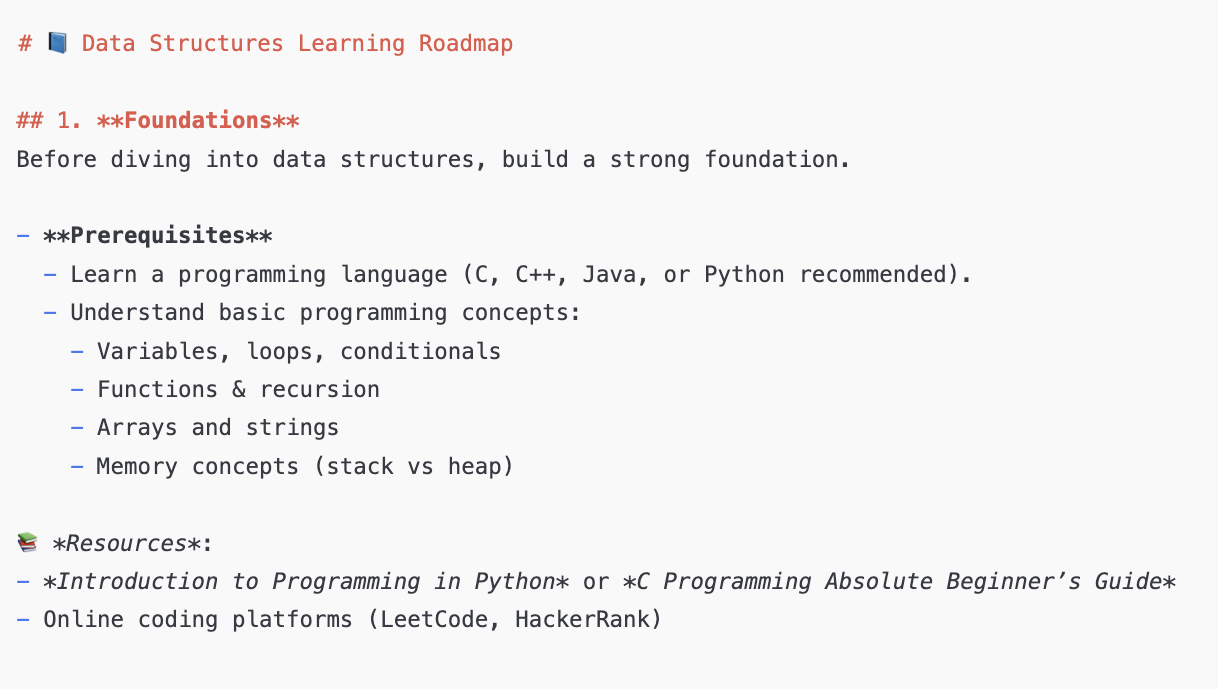
\includegraphics[width=0.8\textwidth]{figures/GPT.png}}
  \end{center}
\end{frame}



\begin{frame}{1.2 Windsurf에서 구체적인 내용 생성}
  \begin{block}{Step 1: 로드맵 불러오기}
    ChatGPT가 생성한 \texttt{Roadmap.md}를 Windsurf에서 불러옴
  \end{block}
  \begin{center}
    \fbox{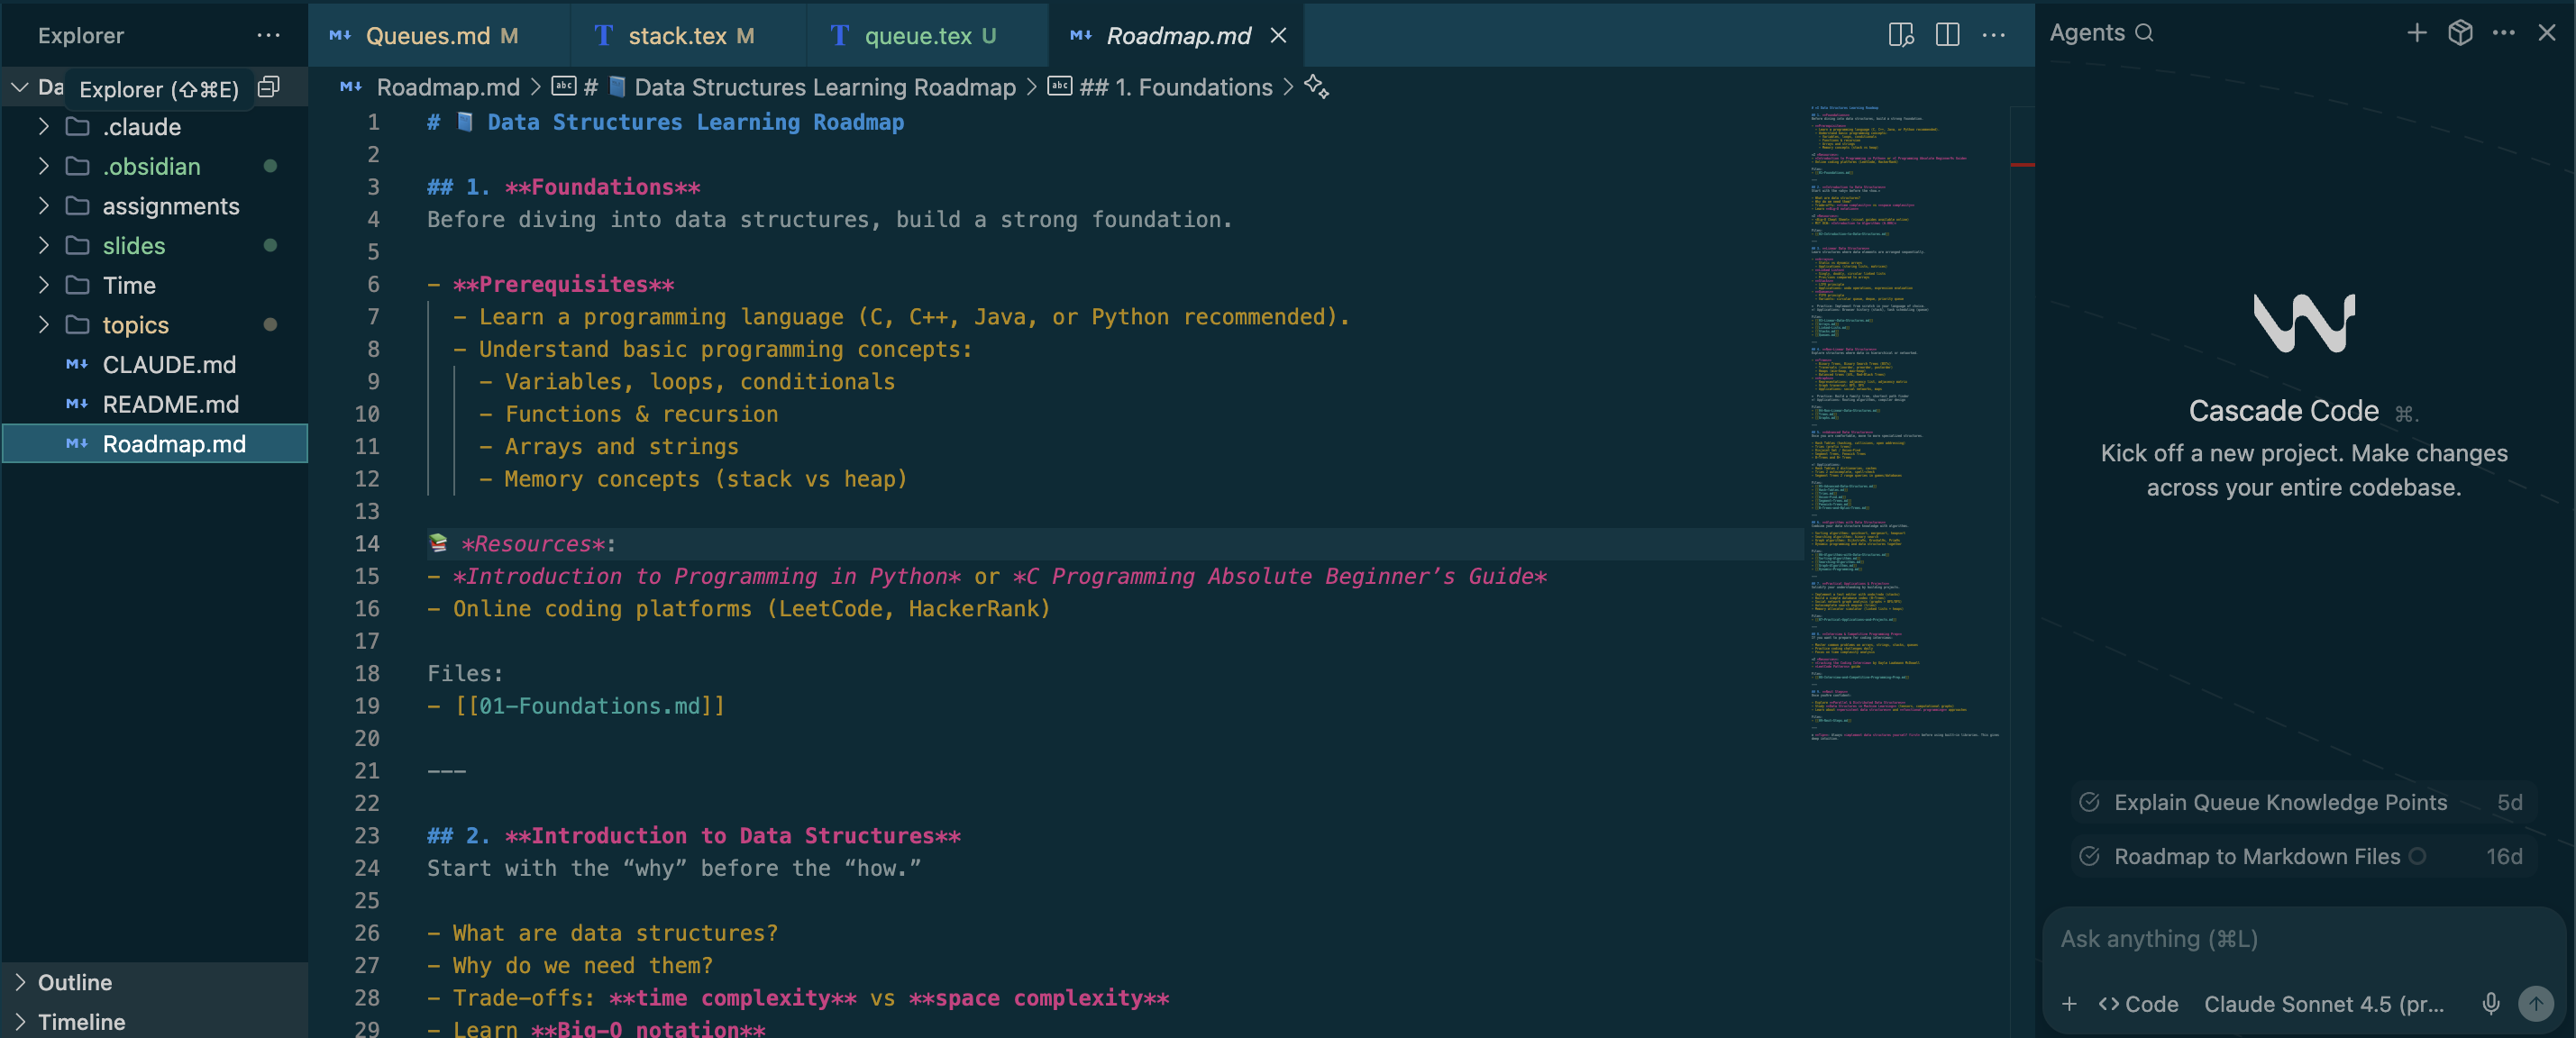
\includegraphics[width=0.9\textwidth]{figures/Windsurf.png}}
  \end{center}
\end{frame}


\begin{frame}{1.2 Windsurf에서 구체적인 내용 생성}

  \begin{block}{Step 2: 단원별 파일 생성}
    AI 채팅에 프롬프트를 입력하여 단원별로 배워야 할 포인트들이 작성된 파일들을 생성
  \end{block}
  \begin{alertblock}{사용한 프롬프트 1}
    % \small
    \textit{``This is a learning roadmap report. I need you todo the following: \\
Step 1. Based on the learning roadmap, create a list of markdown files for each topic.\\  
Step 2. For each topic, write an introduction and list of knowledge points. Each knowlege point title should be written in [[]]''}
  \end{alertblock}

  \begin{alertblock}{사용한 프롬프트 2}
    % \small
    \textit{``I need you to explain the knowledge points in detail''}
  \end{alertblock}

\end{frame}




\begin{frame}{1.2 Windsurf에서 구체적인 내용 생성}

  \begin{block}{최종 결과}
    단원별로 체계적으로 정리된 기반 문헌 파일들이 완성됨
  \end{block}
  \begin{center}
    \fbox{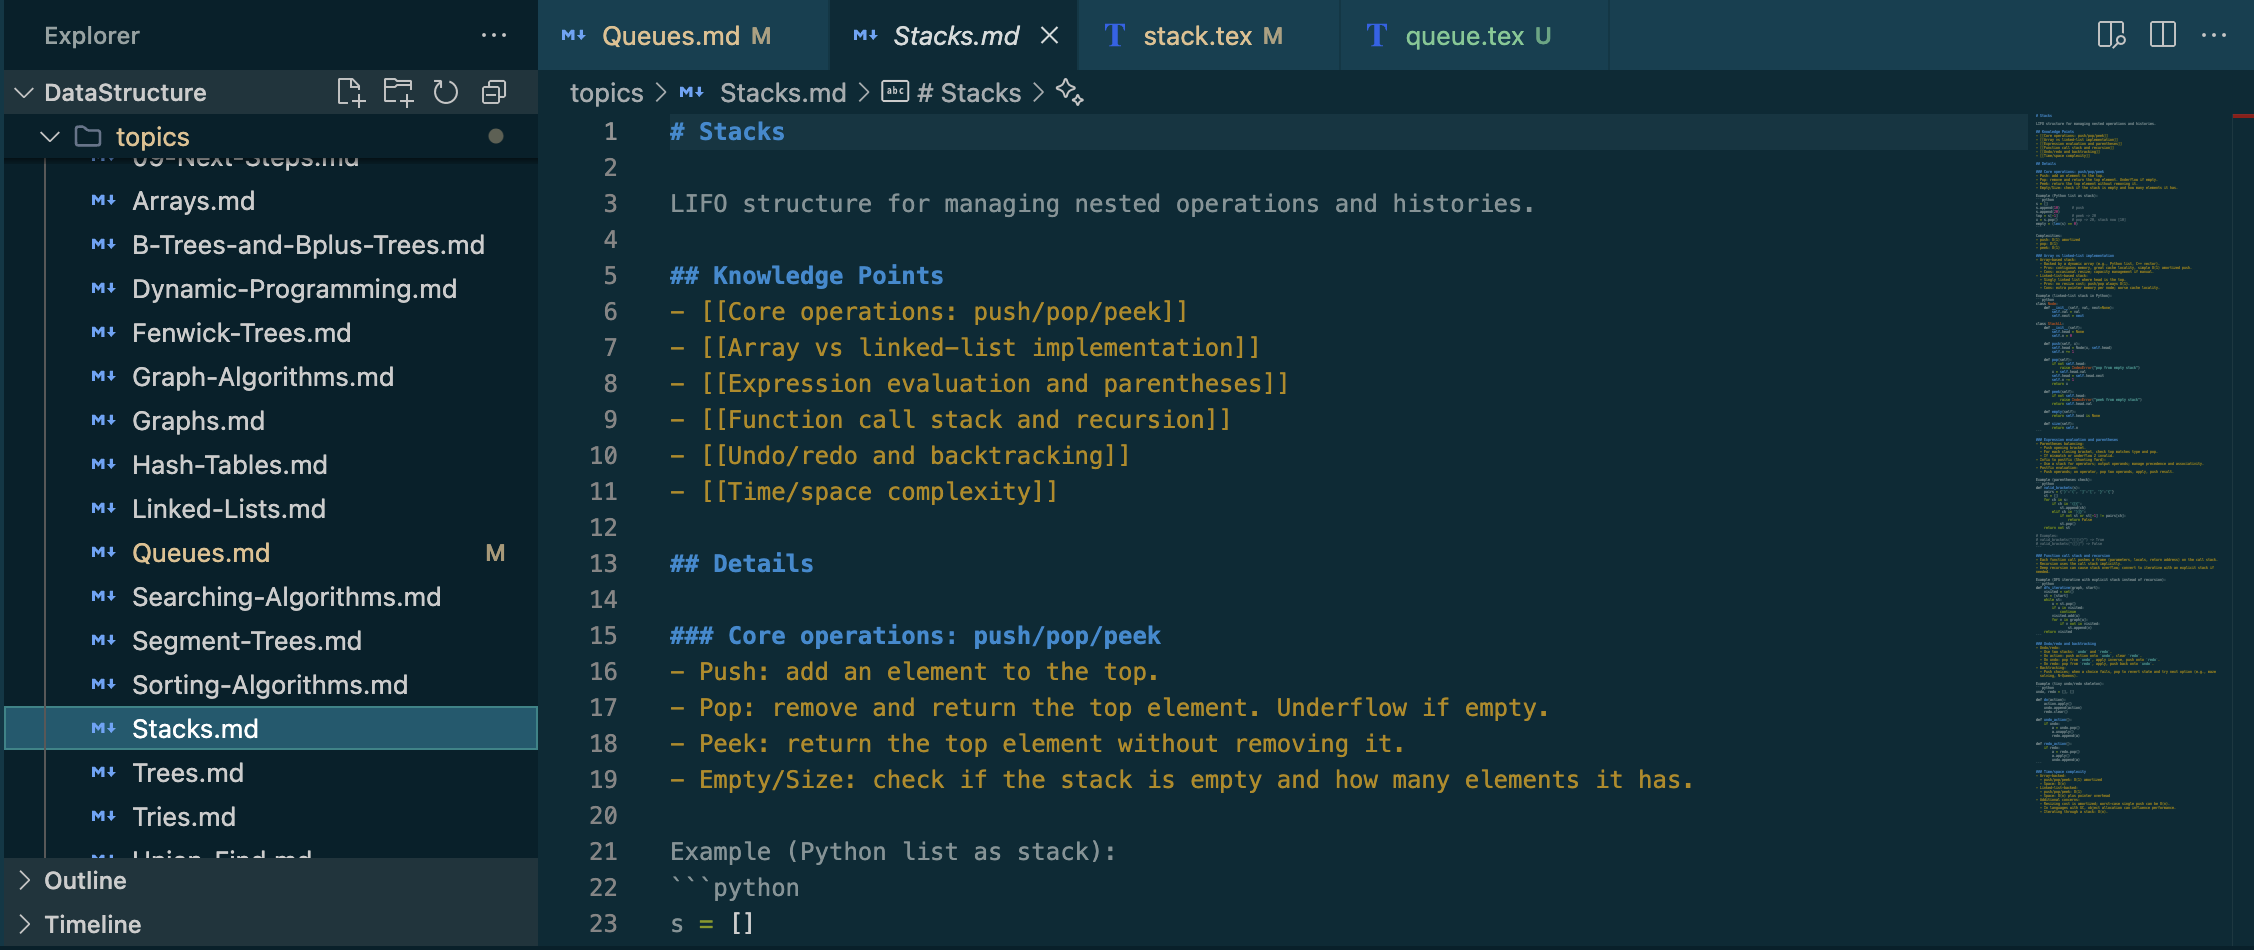
\includegraphics[width=0.9\textwidth]{figures/Stack.png}}
  \end{center}

\end{frame}






\begin{frame}{기반 문헌 생성 결과}
  \begin{center}
    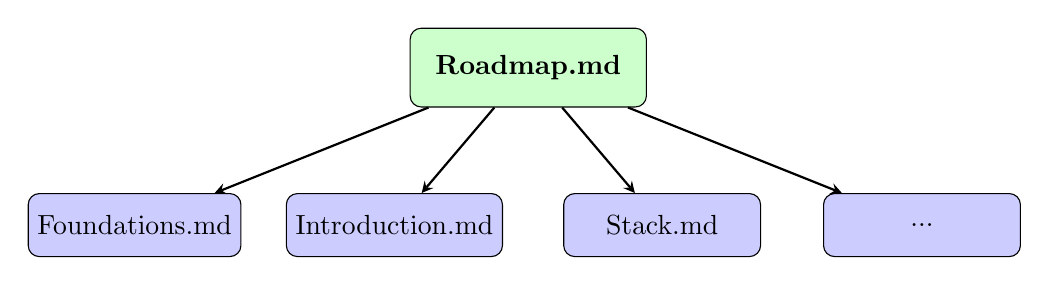
\begin{tikzpicture}
      \node[draw, rounded corners, fill=green!20, minimum width=3cm, minimum height=1cm] (root) at (0,0) {\textbf{Roadmap.md}};

      \node[draw, rounded corners, fill=blue!20, minimum width=2.5cm, minimum height=0.8cm] (topic1) at (-5,-2) {Foundations.md};
      \node[draw, rounded corners, fill=blue!20, minimum width=2.5cm, minimum height=0.8cm] (topic2) at (-1.7,-2) {Introduction.md};
      \node[draw, rounded corners, fill=blue!20, minimum width=2.5cm, minimum height=0.8cm] (topic3) at (1.7,-2) {Stack.md};
      \node[draw, rounded corners, fill=blue!20, minimum width=2.5cm, minimum height=0.8cm] (topic4) at (5,-2) {...};

      \draw[->,>=stealth,thick] (root) -- (topic1);
      \draw[->,>=stealth,thick] (root) -- (topic2);
      \draw[->,>=stealth,thick] (root) -- (topic3);
      \draw[->,>=stealth,thick] (root) -- (topic4);
      % \node[above of=root, node distance=1.5cm] {\Large\textbf{생성된 문헌 구조}};
    \end{tikzpicture}
  \end{center}

  \begin{block}{디렉토리 구조}
    \texttt{DataStructure/}\\
    \hspace{1cm}\texttt{|-- Roadmap.md}\\
    \hspace{1cm}\texttt{|-- topics/}\\
    \hspace{2cm}\texttt{|-- Foundations.md}\\
    \hspace{2cm}\texttt{|-- ...}
  \end{block}
\end{frame}

% %----------------------------------------------------------------------------------------
\section{2단계: 슬라이드 생성}
% %----------------------------------------------------------------------------------------

\begin{frame}{2단계: 슬라이드 생성}
  \begin{block}{목표}
    생성한 문헌을 기반으로 수업 슬라이드 생성하기
  \end{block}

  % \vspace{0.5cm}

  \begin{columns}[t]
    \begin{column}{0.48\textwidth}
      \begin{exampleblock}{추가 사용 도구}
        \textbf{Beamer}
        \begin{itemize}
          \item LaTeX 기반 문서 클래스
          \item 학술 및 전문 발표용 슬라이드 제작
          \item \textbf{코드로 슬라이드를 생성}
        \end{itemize}

        \vspace{0.3cm}

        \textbf{Claude Code}
        \begin{itemize}
          \item Claude AI 기반 코딩 보조 도구
          \item 코드 작성, 수정, 설명, 디버깅 지원
        \end{itemize}
      \end{exampleblock}
    \end{column}

    \begin{column}{0.48\textwidth}
      \begin{alertblock}{작업 순서}
        \begin{enumerate}
          \item \texttt{slides/} 폴더 생성
          \item Beamer 템플릿 위치시키기
          \item Claude Code 실행
          \item \texttt{/init} 명령어로 코드베이스 이해
          \item 슬라이드 생성 프롬프트 입력
        \end{enumerate}
      \end{alertblock}
    \end{column}
  \end{columns}
\end{frame}

\begin{frame}{2.1 슬라이드 생성을 위한 세팅}
  \begin{block}{디렉토리 구조 설정}
    \texttt{DataStructure/}\\
    \hspace{0.5cm}\texttt{|-- Roadmap.md}\\
    \hspace{0.5cm}\texttt{|-- topics/}\\
    \hspace{1cm}\texttt{|-- Foundations.md}\\
    \hspace{1cm}\texttt{|-- ...}\\
    \hspace{0.5cm}\texttt{|-- slides/}\\
    \hspace{1cm}\texttt{|-- template/}\\
  \end{block}

  \vspace{0.5cm}

  \begin{exampleblock}{Claude Code 초기화}
    \begin{enumerate}
      \item Root 폴더(\texttt{DataStructure/})에서 Claude Code 실행
      \item \texttt{/init} 명령어 실행
    \end{enumerate}
  \end{exampleblock}
\end{frame}

\begin{frame}{2.2 Claude Code로 슬라이드 생성}
  \begin{alertblock}{프롬프트}
    Currently, I am teaching Data Structure course based on the markdown files in the 'topics/' folder.\\\vspace{1em}
    In the lecture, I will use slides that are constructed based on the markdown files in the 'topic/' folder.\\\vspace{1em}
    I will use Beamer to generate slides, and the template I will use is placed in the 'slides/BeamerTemplate/' folder.\\\vspace{1em}
    I need you to generate a folder ‘slides/Stack/’ and write a Beamer LaTeX file stack.tex based on the contents in 'topics/Stack.md' and referring to the template in 'slides/BeamerTemplate'.
  \end{alertblock}
\end{frame}



\begin{frame}{2.2 Claude Code로 슬라이드 생성}
  \begin{block}{결과}
    AI에 의해 자동으로 생성된 전문적인 강의 슬라이드
  \end{block}
  \begin{center}
  \fbox{
\includegraphics[width=0.15\textwidth]{figures/Stack/1.png}}
  \fbox{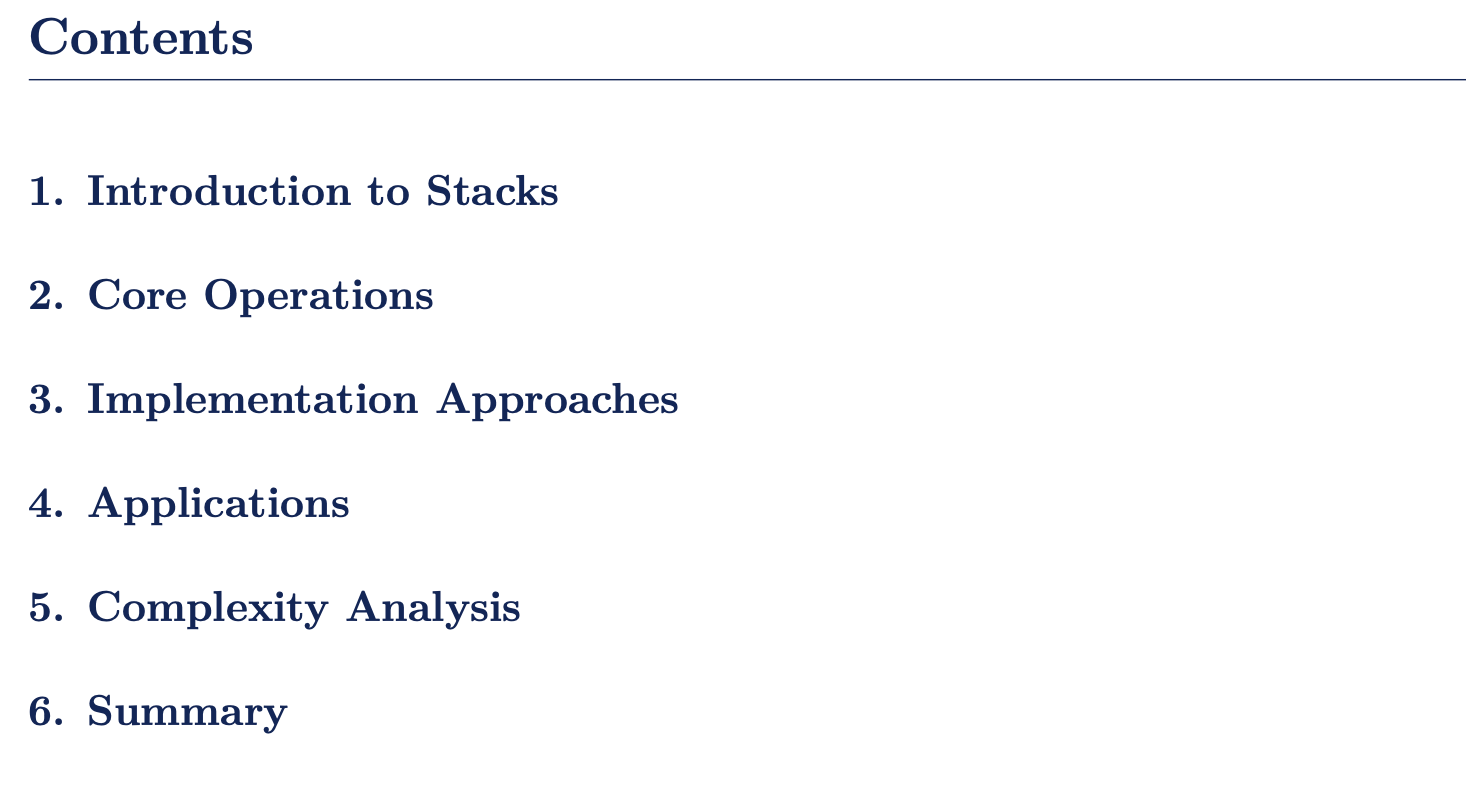
\includegraphics[width=0.15\textwidth]{figures/Stack/2.png}}
  \fbox{
\includegraphics[width=0.15\textwidth]{figures/Stack/3.png}}
  \fbox{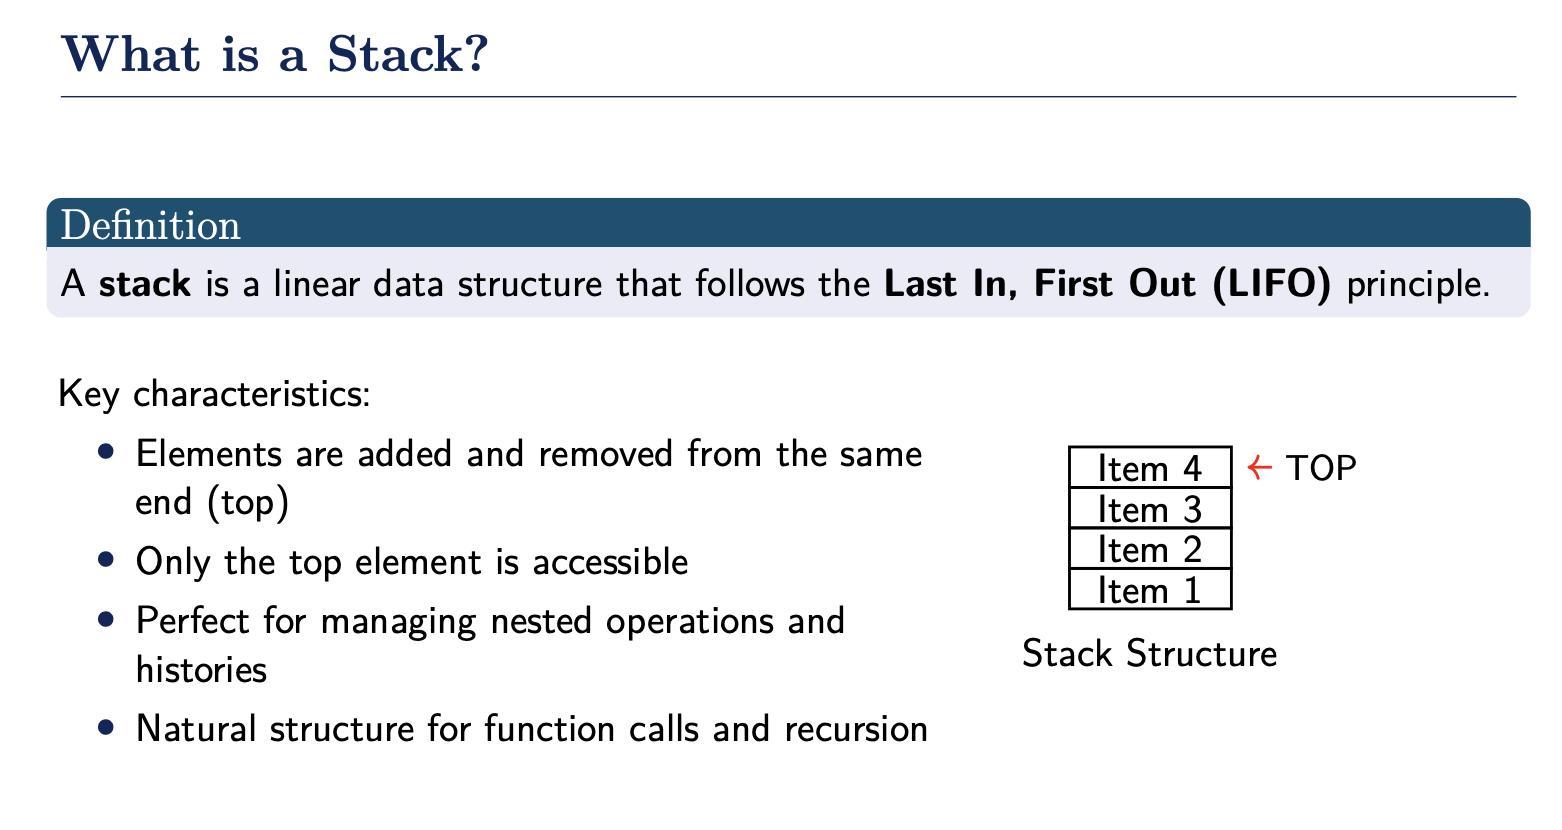
\includegraphics[width=0.15\textwidth]{figures/Stack/4.png}}
  \fbox{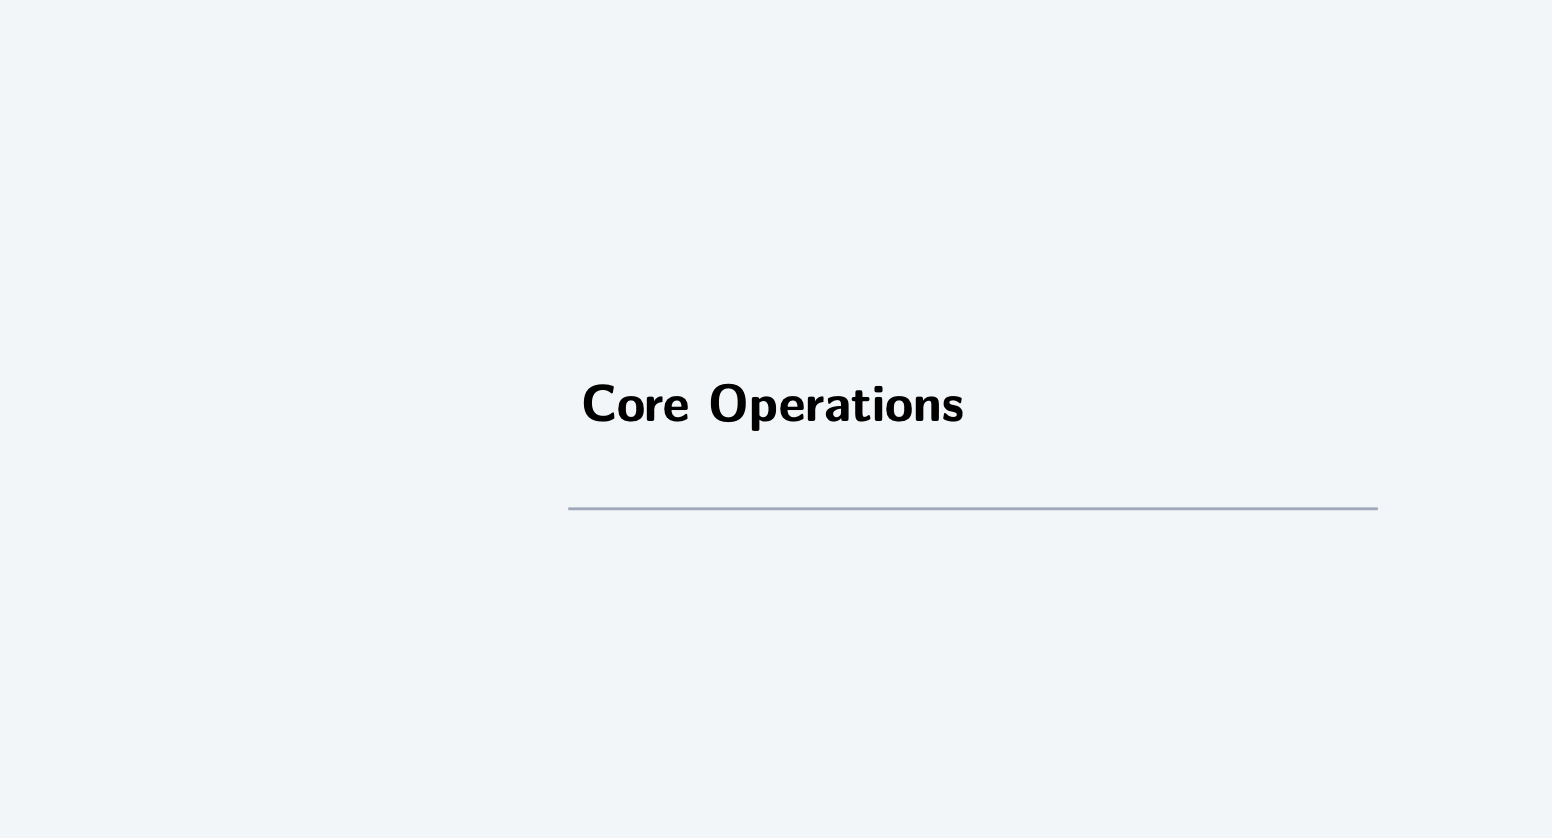
\includegraphics[width=0.15\textwidth]{figures/Stack/5.png}}
  \fbox{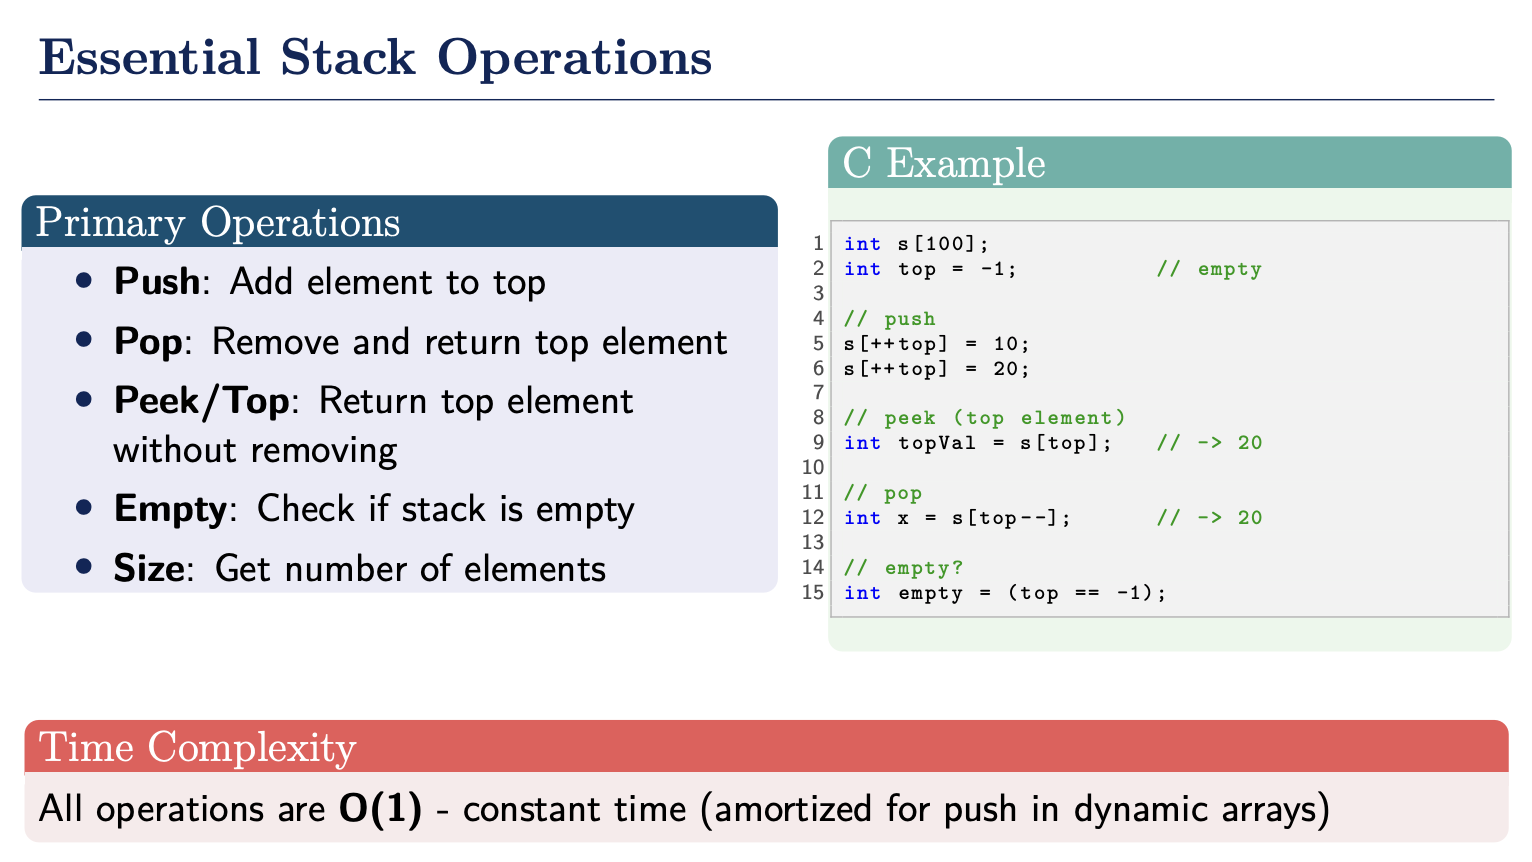
\includegraphics[width=0.15\textwidth]{figures/Stack/6.png}}
  \fbox{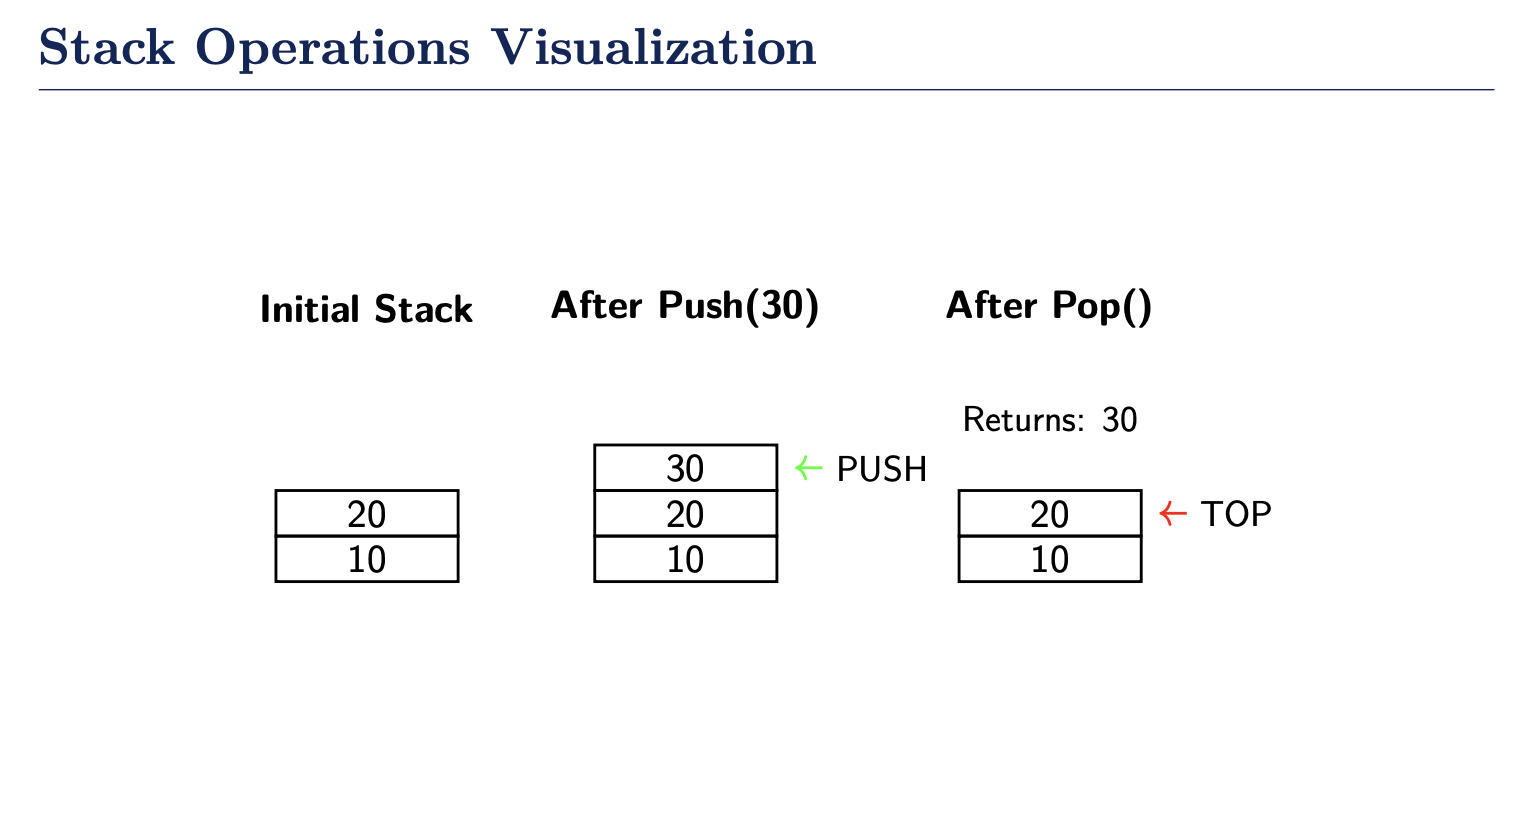
\includegraphics[width=0.15\textwidth]{figures/Stack/7.png}}
  \fbox{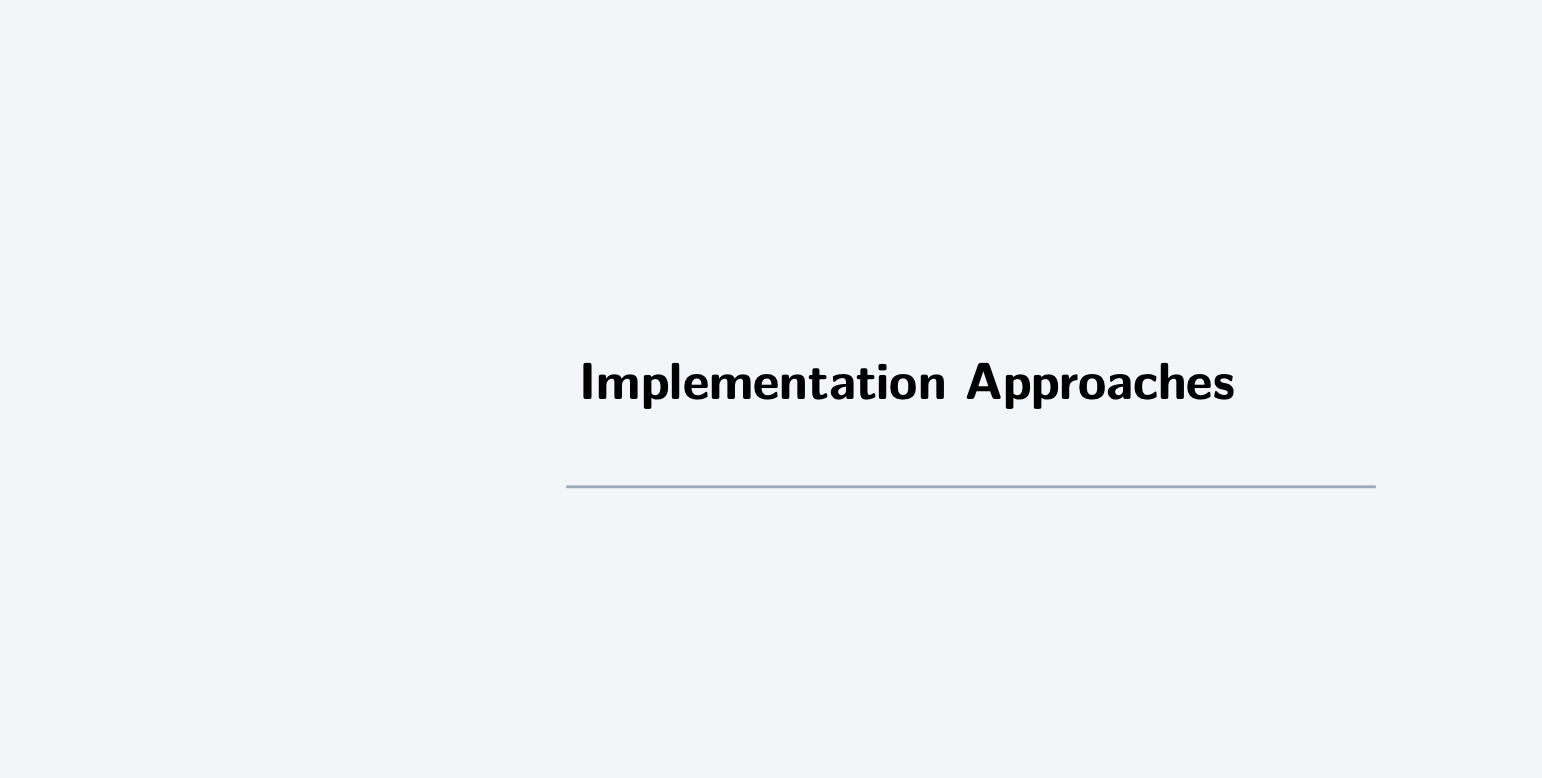
\includegraphics[width=0.15\textwidth]{figures/Stack/8.png}}
  \fbox{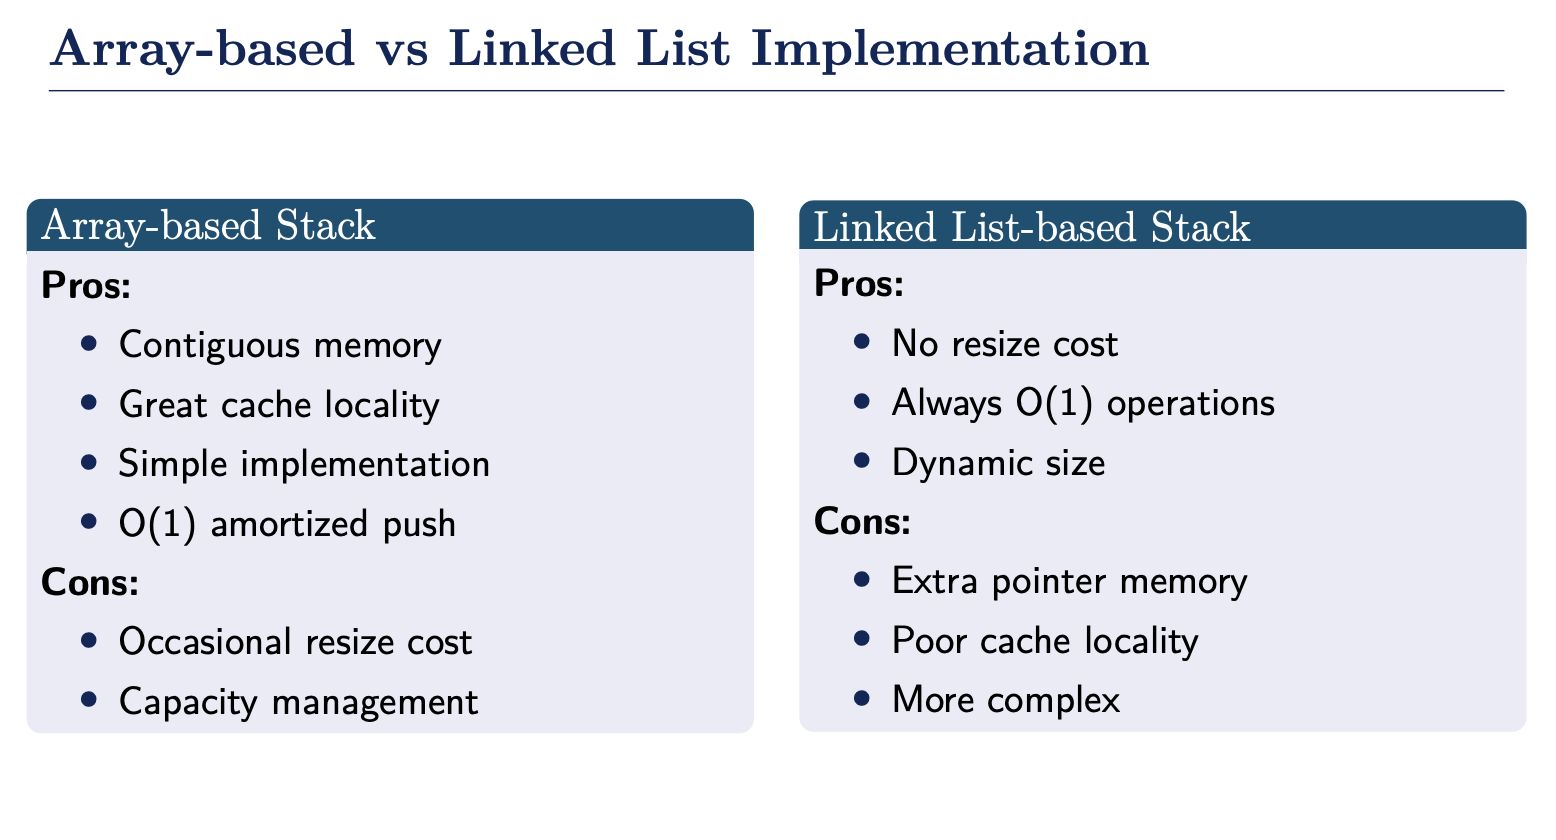
\includegraphics[width=0.15\textwidth]{figures/Stack/9.png}}
  \fbox{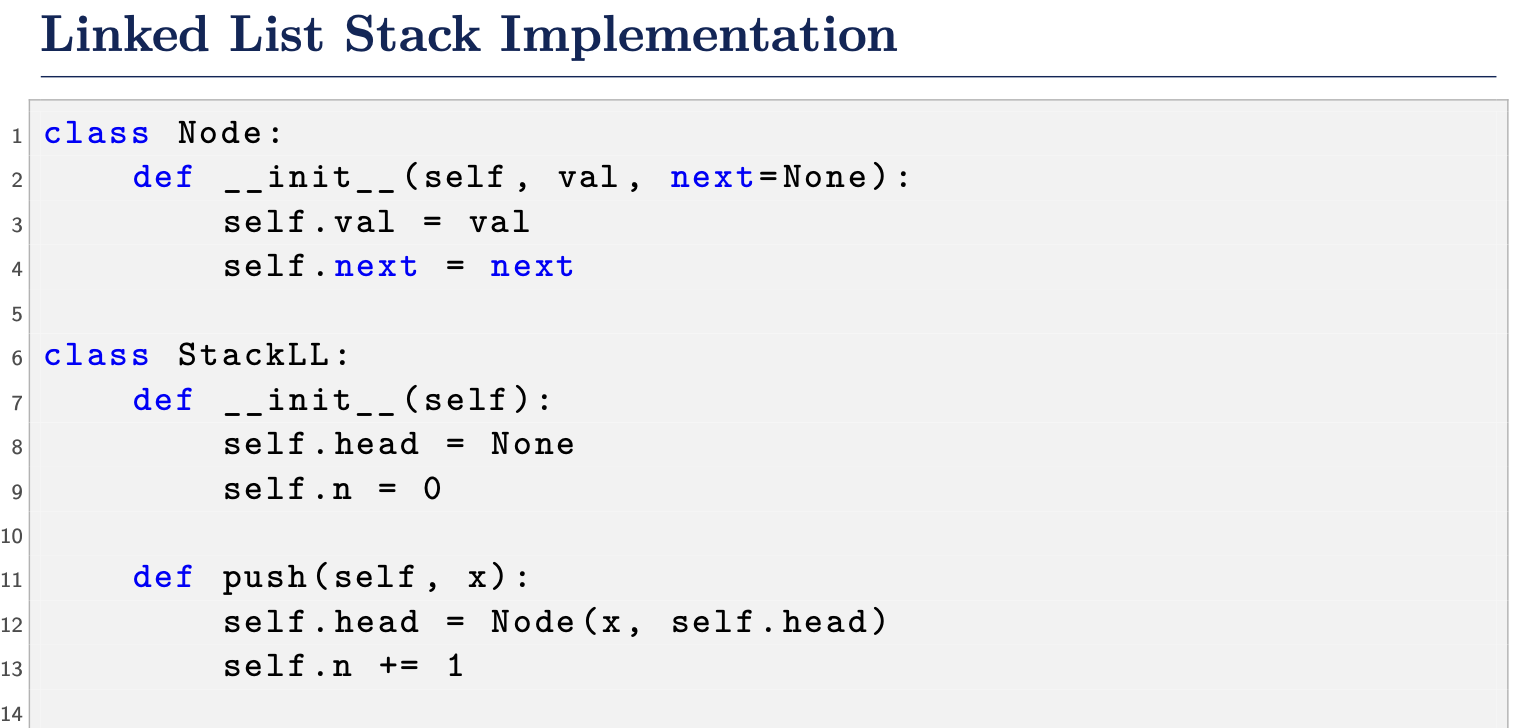
\includegraphics[width=0.15\textwidth]{figures/Stack/10.png}}
  \fbox{
\includegraphics[width=0.15\textwidth]{figures/Stack/11.png}}
  \fbox{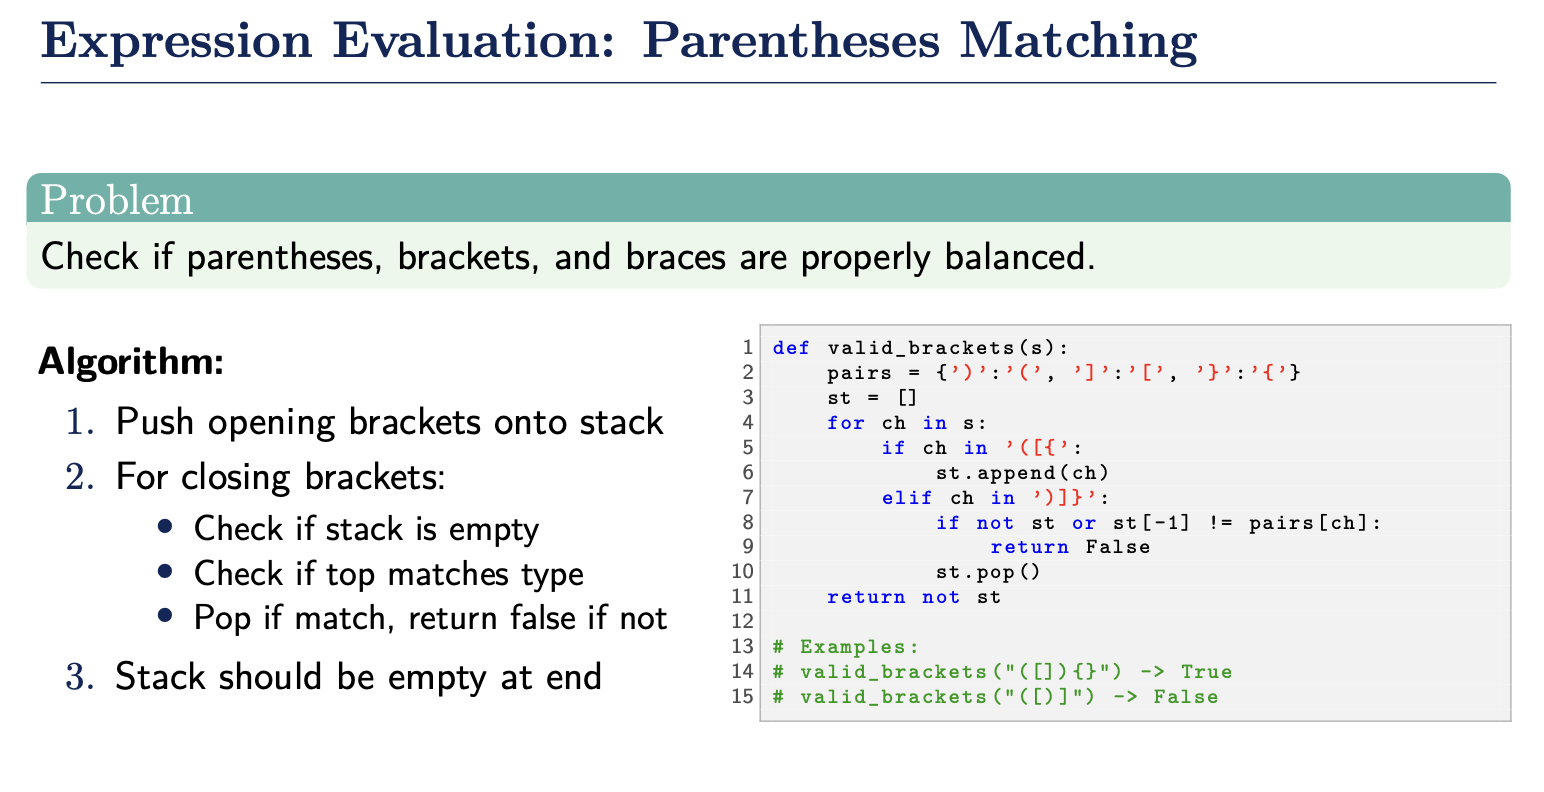
\includegraphics[width=0.15\textwidth]{figures/Stack/12.png}}
  \fbox{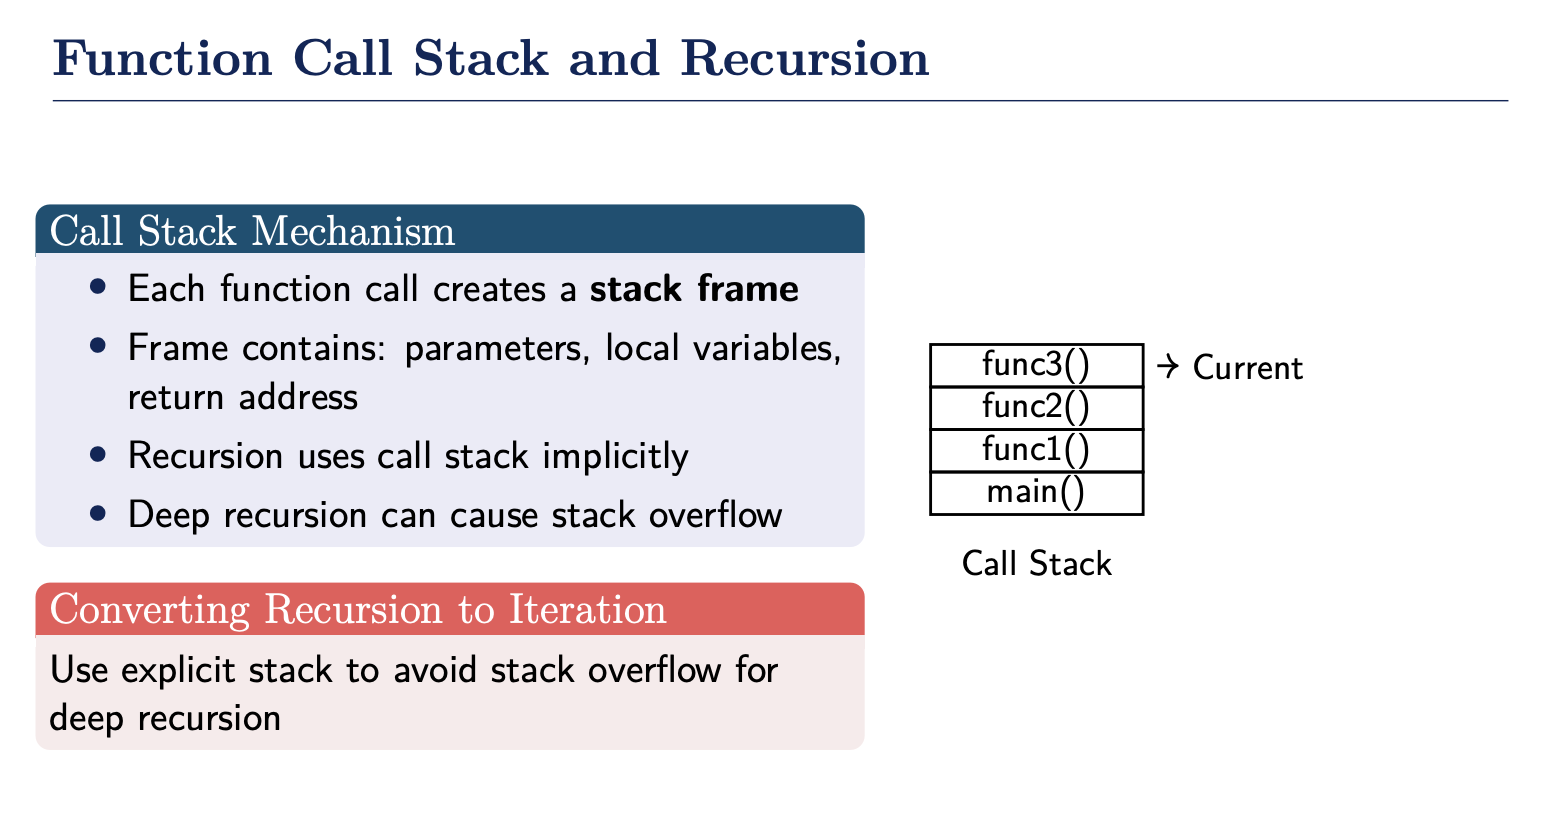
\includegraphics[width=0.15\textwidth]{figures/Stack/13.png}}
  \fbox{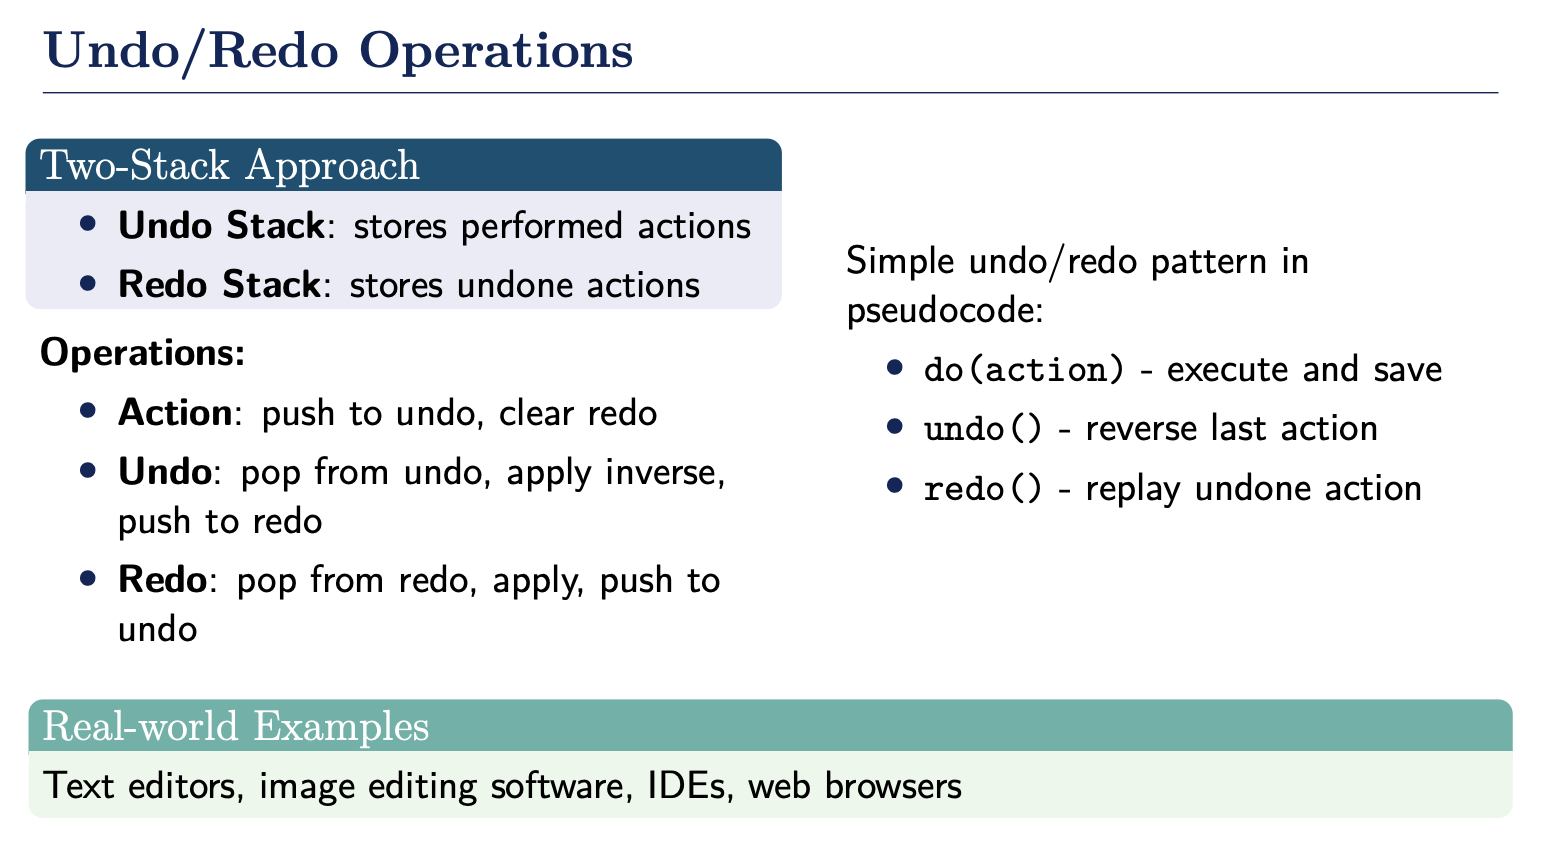
\includegraphics[width=0.15\textwidth]{figures/Stack/14.png}}
  \fbox{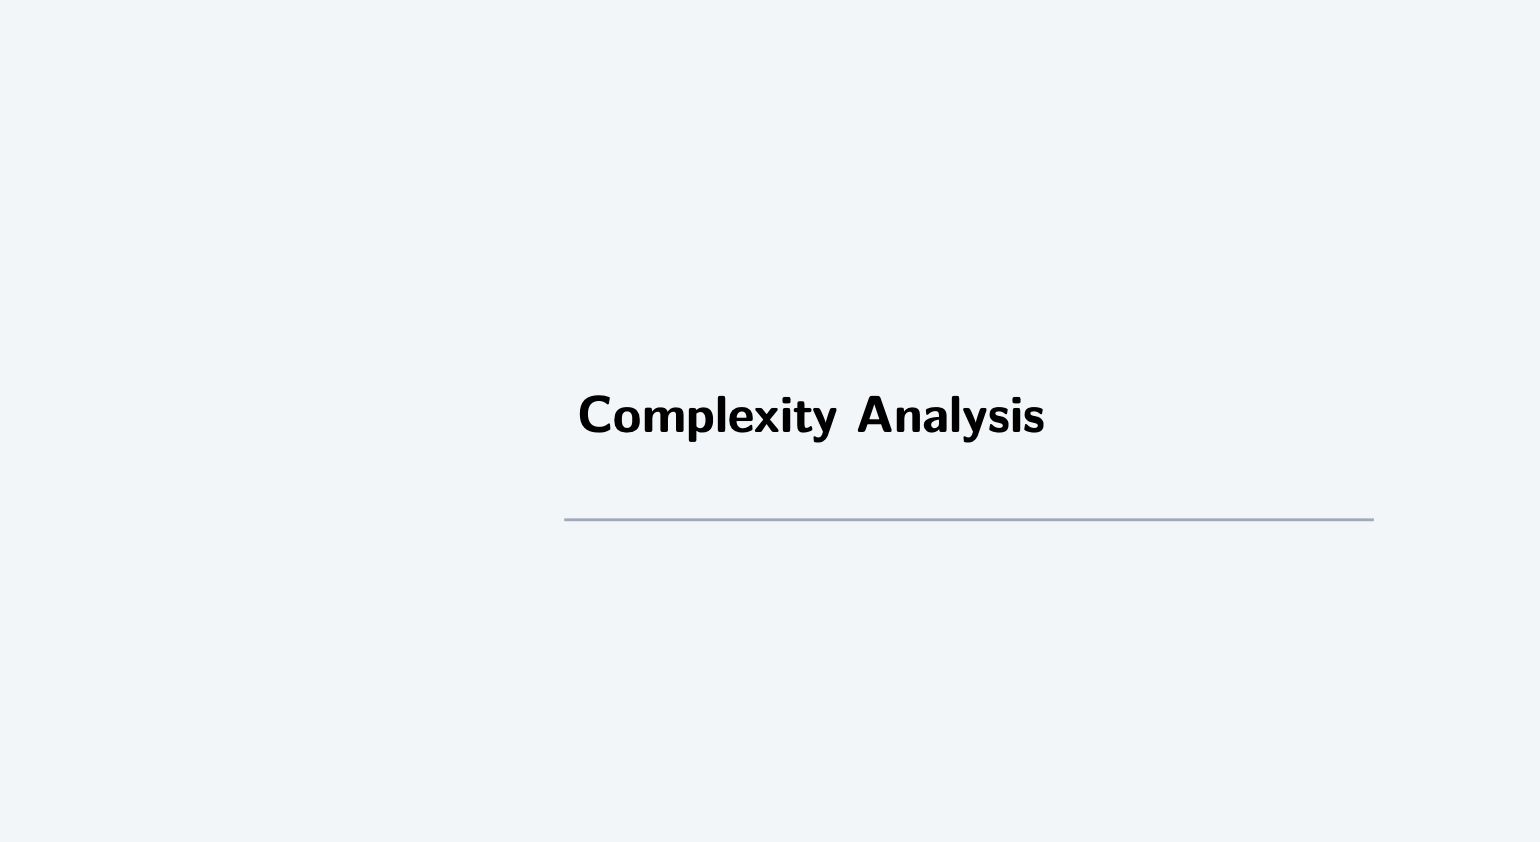
\includegraphics[width=0.15\textwidth]{figures/Stack/15.png}}
  \fbox{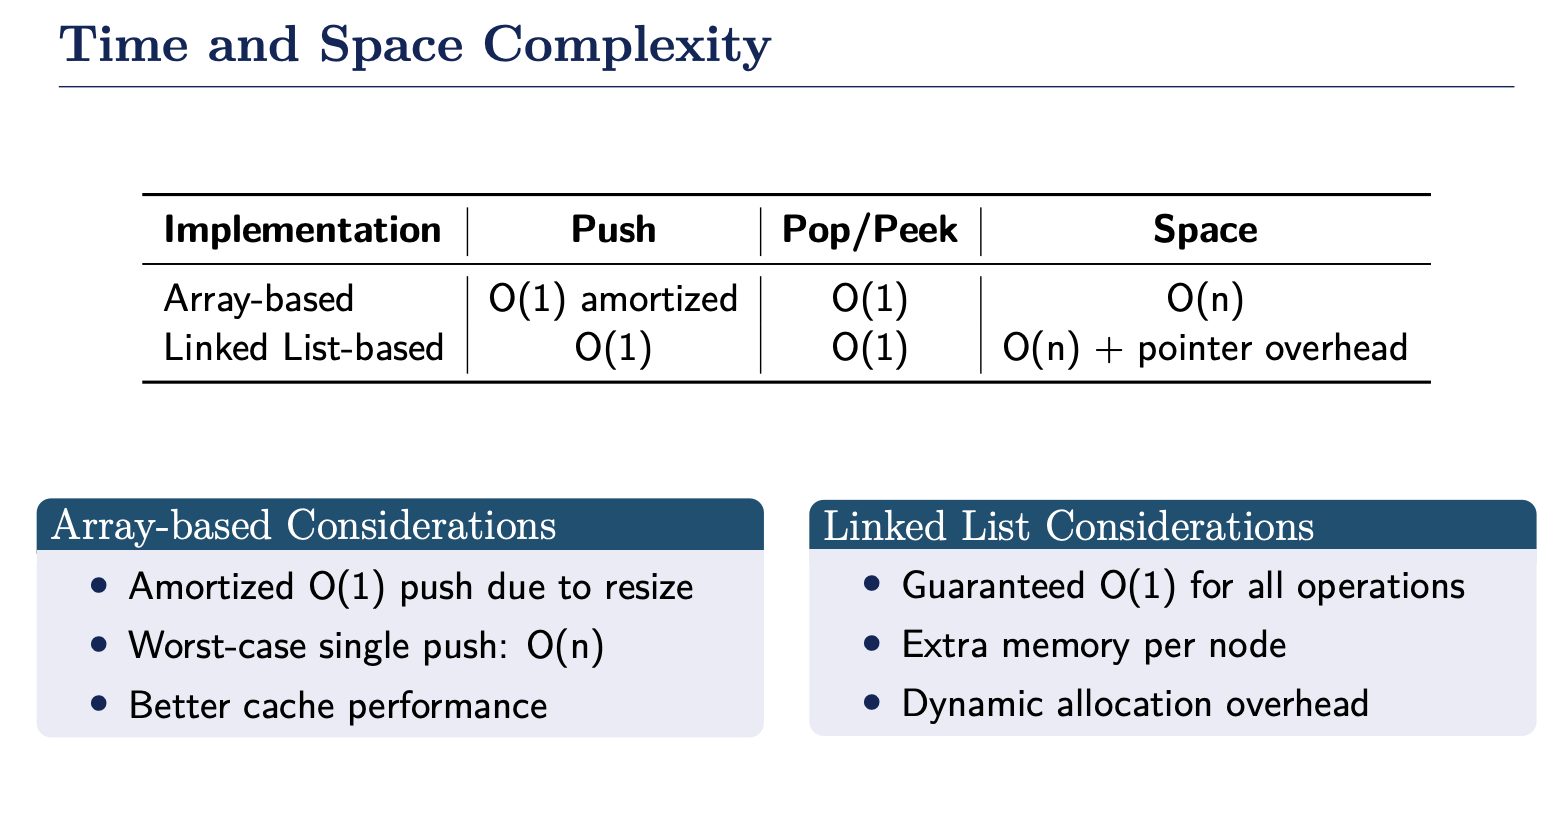
\includegraphics[width=0.15\textwidth]{figures/Stack/16.png}}
  \fbox{
\includegraphics[width=0.15\textwidth]{figures/Stack/17.png}}
  \fbox{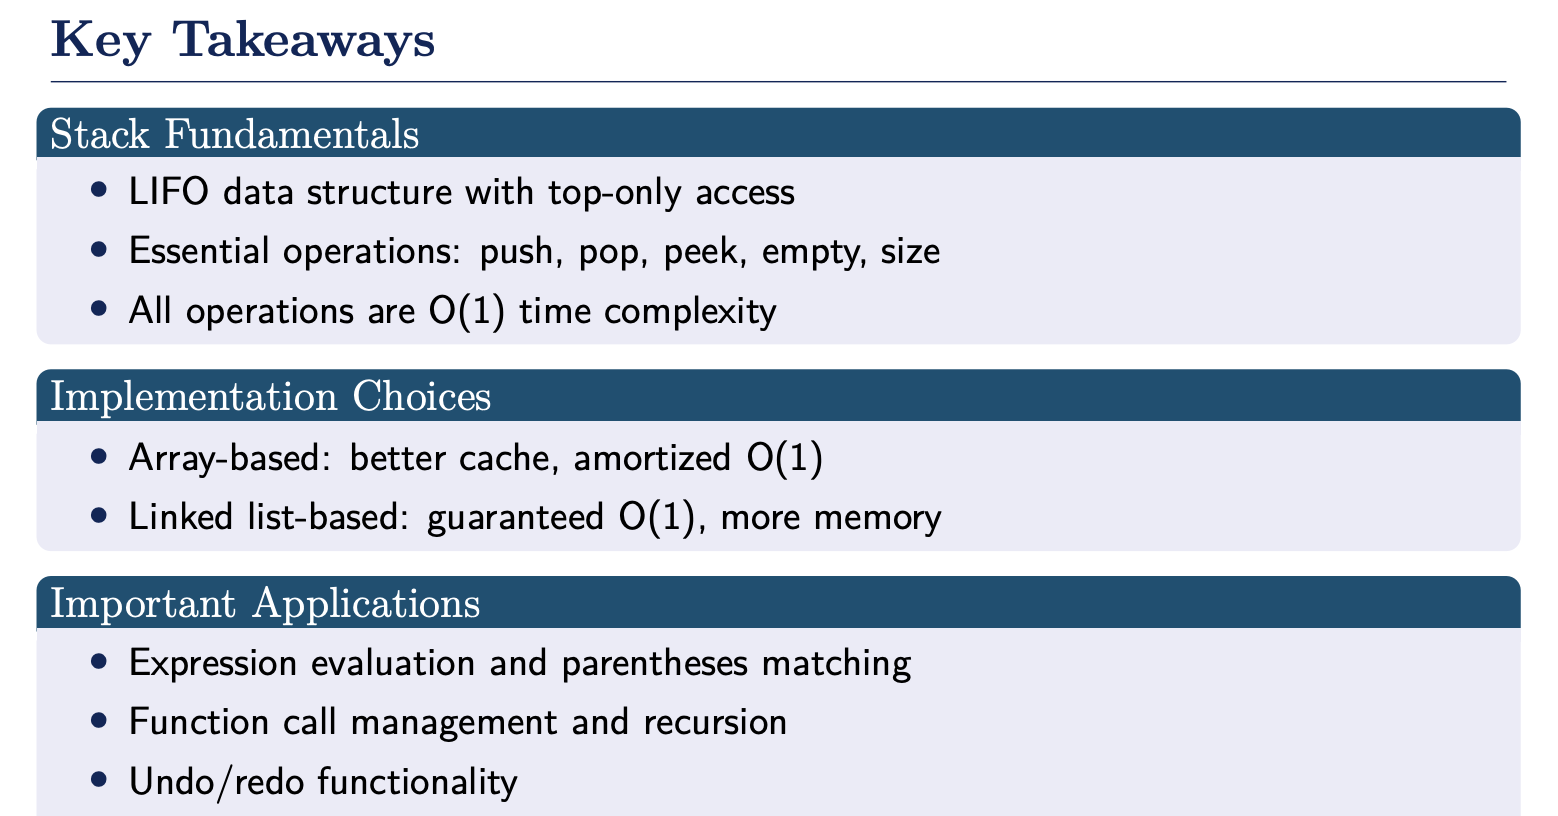
\includegraphics[width=0.15\textwidth]{figures/Stack/18.png}}
  \fbox{
\includegraphics[width=0.15\textwidth]{figures/Stack/19.png}}
  \end{center}
\end{frame}

% 
%----------------------------------------------------------------------------------------
\section{3단계: 과제 생성}
% %----------------------------------------------------------------------------------------

\begin{frame}{3단계: 과제 생성}
  \begin{block}{목표}
    생성한 문헌을 기반으로 과제 생성하기
  \end{block}


  \begin{columns}[t]
    \begin{column}{0.48\textwidth}
      \begin{exampleblock}{디렉토리 구조}
        \texttt{DataStructure/}\\
        \hspace{0.5cm}\texttt{|-- Roadmap.md}\\
        \hspace{0.5cm}\texttt{|-- topics/}\\
        \hspace{0.5cm}\texttt{|-- slides/}\\
        \hspace{0.5cm}\texttt{|-- assignments/}
      \end{exampleblock}
    \end{column}

    \begin{column}{0.48\textwidth}
      \begin{alertblock}{생성 과정}
        \begin{enumerate}
          \item \texttt{assignments/} 디렉토리 생성
          \item Claude Code에 프롬프트 입력
          \item 문헌 및 슬라이드 기반 과제 생성
        \end{enumerate}
      \end{alertblock}
    \end{column}
  \end{columns}

\end{frame}


\begin{frame}{3단계: 과제 생성}

  \begin{alertblock}{프롬프트}
    Currently, I am teaching Data Structure course based on the markdown files in the 'topics/' folder.\\\vspace{1em}
    In the lecture, I will give the students assignments about implementing each data structure. \\\vspace{1em}
    I need you to generate ‘assignments/stack’ folder and implement ‘stack.py’ that implements the core functions of stack data structure, and also write an application code ‘application.py’ that imports and uses the functions in stack.py.\\\vspace{1em}
    After you implement the core functions in stack.py, I will hide them and make the student implement them as their assignments.
  \end{alertblock}
\end{frame}

\begin{frame}{3단계: 과제 생성}
  \begin{block}{결과}
    자동으로 생성된 체계적인 과제
  \end{block}
  \fbox{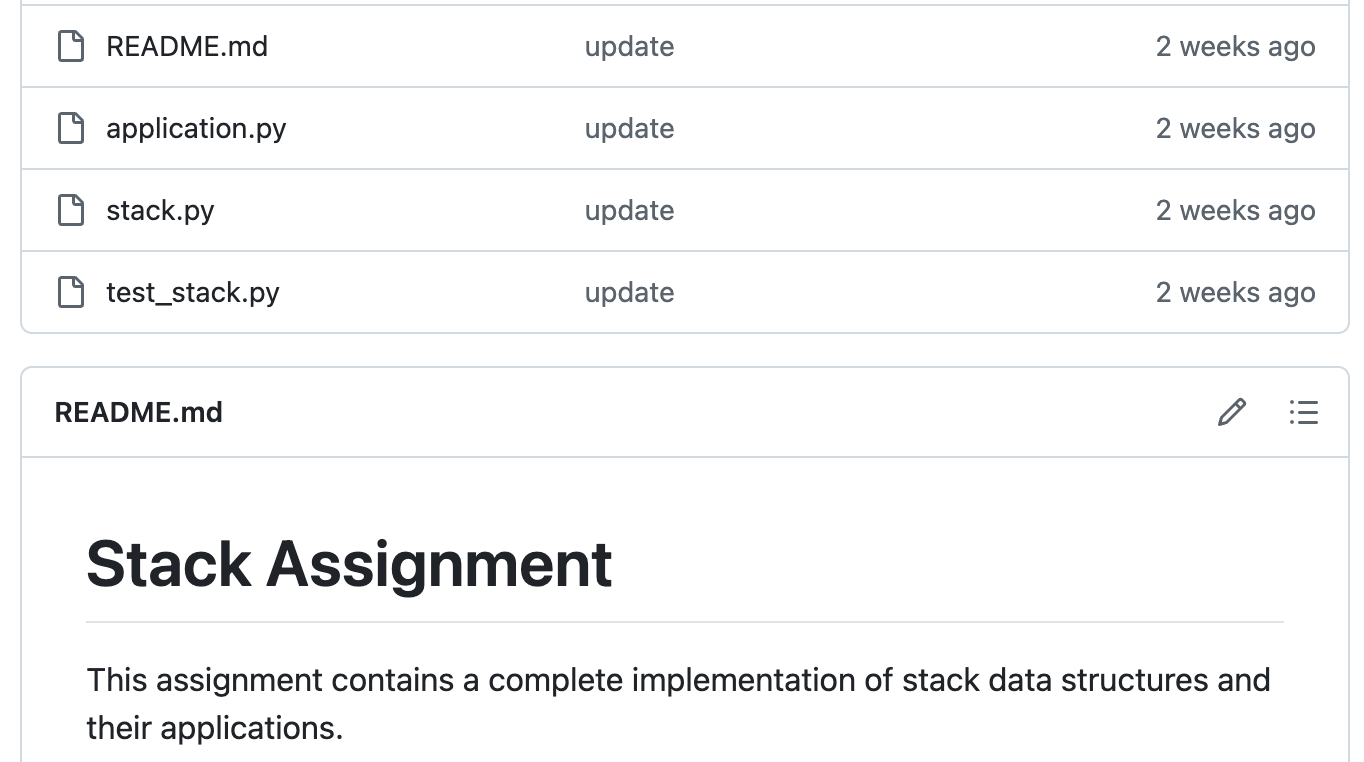
\includegraphics[width=0.5\textwidth]{figures/Assignment.png}}
  \fbox{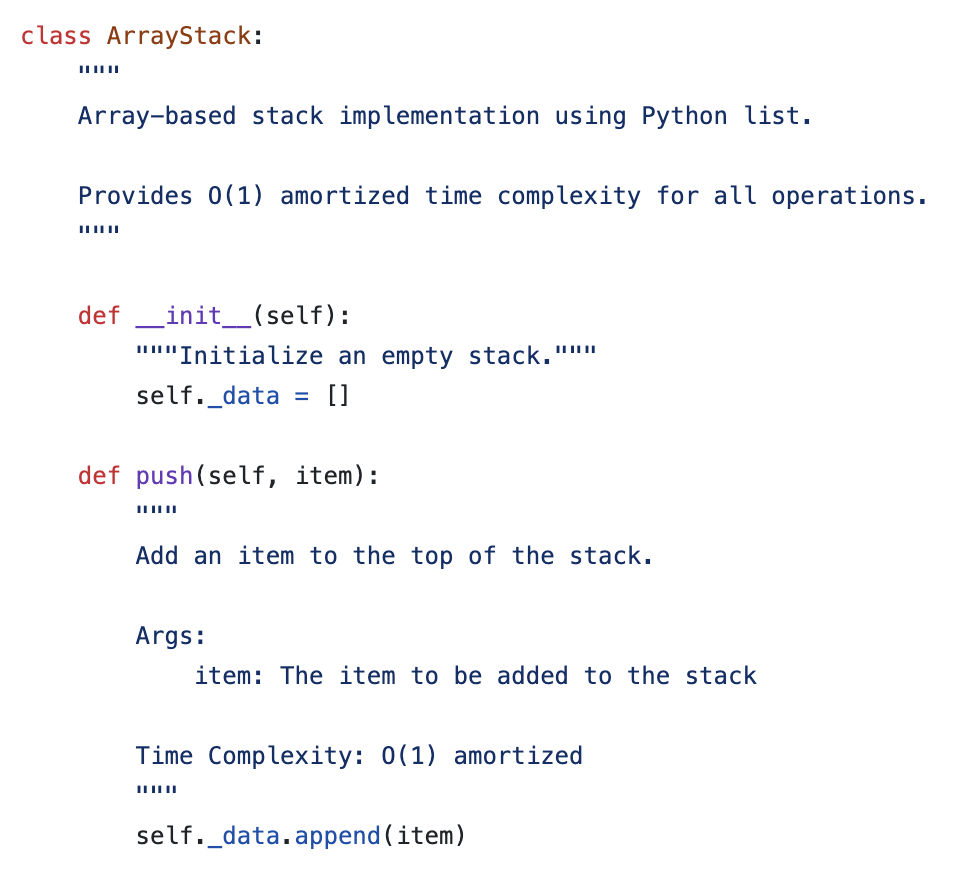
\includegraphics[width=0.4\textwidth]{figures/code.png}}  
\end{frame}

% % %----------------------------------------------------------------------------------------
% \section{4단계: 원격 저장소 관리}
% % %----------------------------------------------------------------------------------------

% \begin{frame}{4단계: 원격 저장소를 통한 관리}
%   \begin{block}{버전 관리 및 협업}
%     생성한 자료들을 원격 저장소(GitHub)를 통해 유지보수
%   \end{block}

%   \vspace{0.5cm}

%   \begin{exampleblock}{장점}
%     \begin{itemize}
%       \item \textbf{버전 관리}: 자료의 변경 이력 추적
%       \item \textbf{백업}: 클라우드 기반 안전한 보관
%       \item \textbf{협업}: 다른 교수자와 자료 공유 및 공동 개발
%       \item \textbf{재사용성}: 다음 학기에도 쉽게 접근 및 수정 가능
%       \item \textbf{공개/비공개 선택}: 필요에 따라 접근 권한 설정
%     \end{itemize}
%   \end{exampleblock}

%   \vspace{0.3cm}

%   \begin{alertblock}{Git 워크플로우}
%     \texttt{git add} → \texttt{git commit} → \texttt{git push}
%   \end{alertblock}
% \end{frame}

% %----------------------------------------------------------------------------------------
% \section{결과물 활용}
% %----------------------------------------------------------------------------------------

% \begin{frame}{학내 적용 방안}
%   \begin{columns}[t]
%     \begin{column}{0.48\textwidth}
%       \begin{block}{교직원 활용}
%         \begin{itemize}
%           \item \textbf{수업 자료의 초안을 빠르게 생성}
%           \item 자동 생성된 초안을 기반으로 보완
%           \item 고품질 수업 자료를 학생들에게 제공
%           \item \textbf{수업의 품질을 비약적으로 향상}
%         \end{itemize}
%       \end{block}
%     \end{column}

%     \begin{column}{0.48\textwidth}
%       \begin{block}{학생 활용}
%         \begin{itemize}
%           \item \textbf{자기 주도 학습} 지원
%           \item 개인 또는 스터디 그룹에서 활용
%           \item \textbf{본인만을 위한 학습 프레임워크} 구축
%           \item 맞춤형 학습 자료 생성
%         \end{itemize}
%       \end{block}
%     \end{column}
%   \end{columns}

%   \vspace{0.5cm}

%   \begin{exampleblock}{기대 효과}
%     \begin{center}
%       \textbf{교육의 질 향상} + \textbf{시간 절약} + \textbf{맞춤형 교육}
%     \end{center}
%   \end{exampleblock}
% \end{frame}

% %----------------------------------------------------------------------------------------
% \section{결론}
% %----------------------------------------------------------------------------------------

\begin{frame}{결론}
  \begin{block}{AI 기반 수업자료 생성 시스템의 핵심}
    \begin{enumerate}
      \item \textbf{기반 문헌 생성}: ChatGPT + Windsurf로 체계적인 교재 작성
      \item \textbf{슬라이드 생성}: Claude Code + Beamer로 전문적인 프레젠테이션 제작
      \item \textbf{과제 생성}: AI 기반 맞춤형 과제 자동 생성
    \end{enumerate}
  \end{block}

  \vspace{0.5cm}

  \begin{exampleblock}{핵심 가치}
    \begin{center}
      \Large
      효율성 $\times$ 품질 $\times$ 확장성
    \end{center}
  \end{exampleblock}

  \vspace{0.3cm}

  \begin{alertblock}{향후 전망}
    AI 기술의 발전과 함께 더욱 정교하고 개인화된 교육 자료 생성 가능
  \end{alertblock}
\end{frame}

\begin{frame}[plain]
  \centering
  \Huge \textbf{감사합니다!}

  \vspace{1cm}
  \normalsize
  질문이 있으시면 언제든지 말씀해주세요.\\\vspace{1em}
  
  참고 자료: \href{https://github.com/MinseokJGit/DataStructure/tree/main}{https://github.com/MinseokJGit/DataStructure/}
\end{frame}

\end{document}
